\documentclass[12]{report}
\usepackage[utf8]{inputenc}
\usepackage[T1]{fontenc}
\usepackage[francais]{babel}
\usepackage{listings}
\usepackage{hyperref}
\usepackage{graphicx}
\usepackage{caption}
\usepackage{xcolor}
\usepackage{titlepic}

\definecolor{denim}{rgb}{0.08, 0.38, 0.74}

\hypersetup{
  colorlinks=true,
  linktoc=all,
  linkcolor=denim,
}
\title{\textbf{Projet de communication transdisciplinaire \\ Rapport}}
\author{Mahazoasy Heritiana, Jalenques Hugo, Dupland Erwan, Tremor Suulyvan}
\date\today{}
\titlepic{
\includegraphics[height=3.5cm]{ub.png}
\hfill

\includegraphics[height=3.5cm]{mba.png}}


\begin{document}
\renewcommand{\contentsname}{Sommaire}

\maketitle
\tableofcontents

  \chapter{Introduction}

  Afin de se développer, le musée des Beaux Arts de Bordeaux a besoin d'informations sur ses visiteurs. Jusqu'à maintenant, le musée a mis en place des études de publics ponctuelles et irrégulières. Mais le recueil de données sur les visiteurs à travers ces questionnaires contrarie le public.
  \\

  Le musée des Beaux Arts souhaite donc mettre en place un outil numérique à disposition des visiteurs qui lui permettrait de recueillir ces données d'une manière ludique et spontanée. \\

  Nous avons donc décider de mettre en place une tablette à l'entrée du musée permettant aux visiteurs de répondre à un questionnaire. Ce questionnaire permettra au musée de récolter des renseignements sur les visiteurs avec des questions de base et permettra aux visiteurs de s'amuser grâce à des questions ludiques.

  \chapter{Besoins et contraintes}

  \section{Expressions des besoins}

  \subsection{Besoins fonctionnels}

  \begin{itemize}
    \item Il faut que le musée puisse recueillir facilement et de manière sécurisée et anonyme les renseignements sur les visiteurs dans une base de donnée extérieure à l'application.
    \item Le musée doit également garder l'anonymat des visiteurs qui remplissent le questionnaire.
  \end{itemize}

  \subsection{Besoins non-fonctionnels}

  \begin{itemize}
    \item Il faut que n'importe quel visiteur puisse utiliser cette tablette.
          Elle doit être facile d'utilisation pour toutes les personnes initiées ou non aux nouvelles technologies, et pour toutes les nationnalités.

    \item Il ne faut pas que le visiteur sente qu'il participe à un \emph{sondage} mais qu'il prenne du plaisir à répondre aux questions en s'amusant par exemple.
    \item Le principe doit être compris rapidement sans demander de connaissances particulières de la part de l'utilisateur pour avoir un maximum de données.
    \item Les informations recueillies doivent apporter des renseignements utiles au client.
  \end{itemize}

  \section{Contraintes}

  L'application ne doit utiliser des éléments graphiques (peintures, ...) appartenant uniquement au Musée des Beaux-Arts. \\

  De plus, l'application doit être ludique et simple d'utilisation pour les visiteurs.

  \chapter{Solution proposée}

  Pour cela, nous sommes partis sur un quiz simple d'utilisation avec une question écrite en haut de l'écran, les propositions en dessous, un bouton \emph{Valider}, un bouton \emph{Annuler} et un bouton {Retour}.

  Le quiz sera lié à une base de données facilement exportable à l'aide d'un bouton.

  \newpage
  \section{Le Quiz}

  À travers une alternance de quesions ludiques et d'autres plus formelles, le quiz récupère les informations suivantes sur les visiteurs :

  \begin{itemize}
    \item Âge
    \item Sexe
    \item Niveau scolaire
    \item Nationalité
    \item Première visite
    \item Présence d'enfants
    \item Mode de découverte du musée
    \item Niveau de satisfaction
    \item Recommandation \\
  \end{itemize}

  Il laisse aussi la possibilité de laisser un commentaire personnel. \\

  \section{Application}

  \begin{center}
    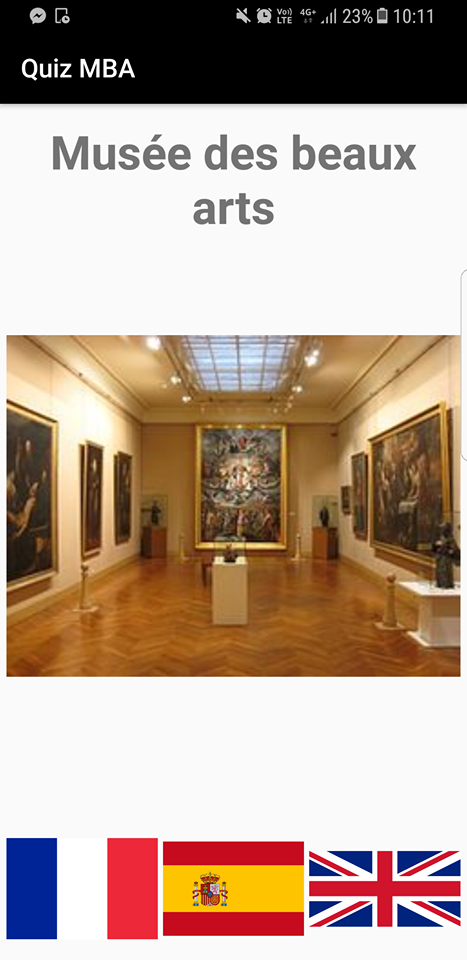
\includegraphics[width=5cm]{menu.png}
    \captionof{figure}{Menu de l'application}
  \end{center}

  Il est possible d'effectuer le questionnaire en plusieurs langues, il suffit simplement de cliquer sur le drapeau correspondant. \\


  \begin{center}
    
\includegraphics[width=3.8cm]{age_fr.png}
    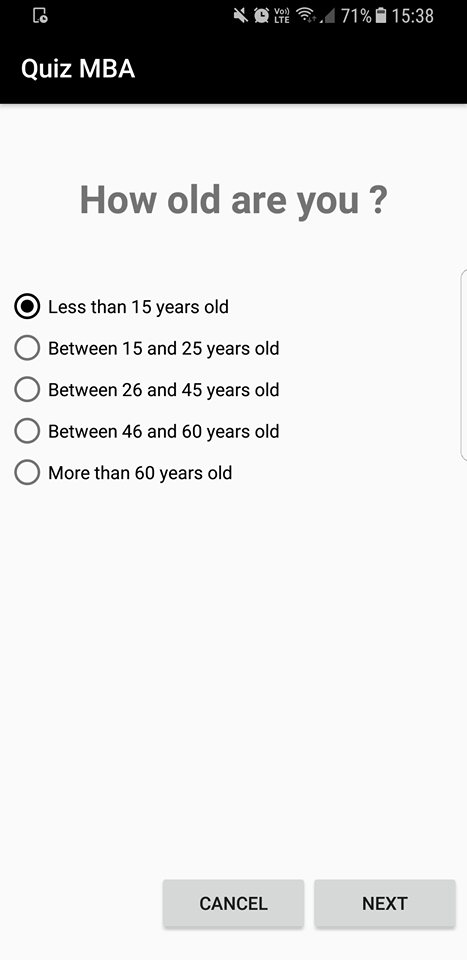
\includegraphics[width=3.8cm]{age_an.png}
    
\includegraphics[width=3.8cm]{age_es.png}
    \captionof{figure}{Illustration des différentes langues}
  \end{center}

  Différents type de questions : choix multiples, curseur, symbole et commentaire. \\

  \begin{center}
    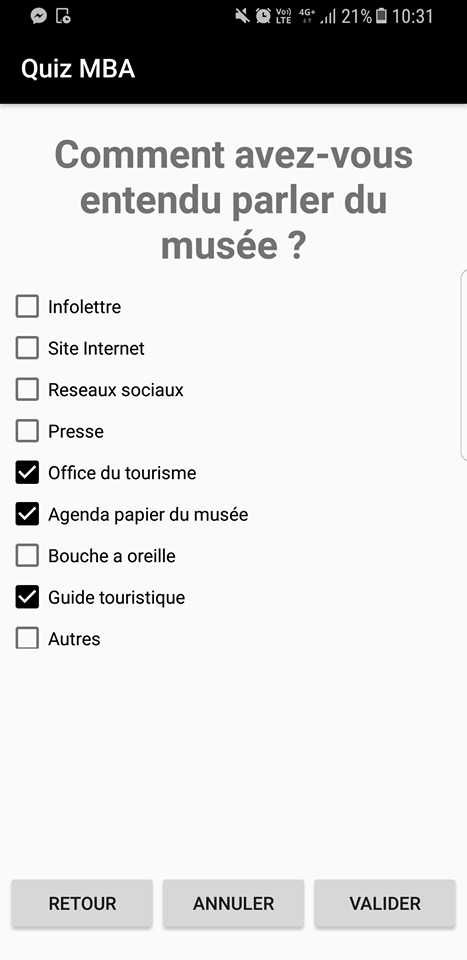
\includegraphics[width=2.8cm]{musee.png}
    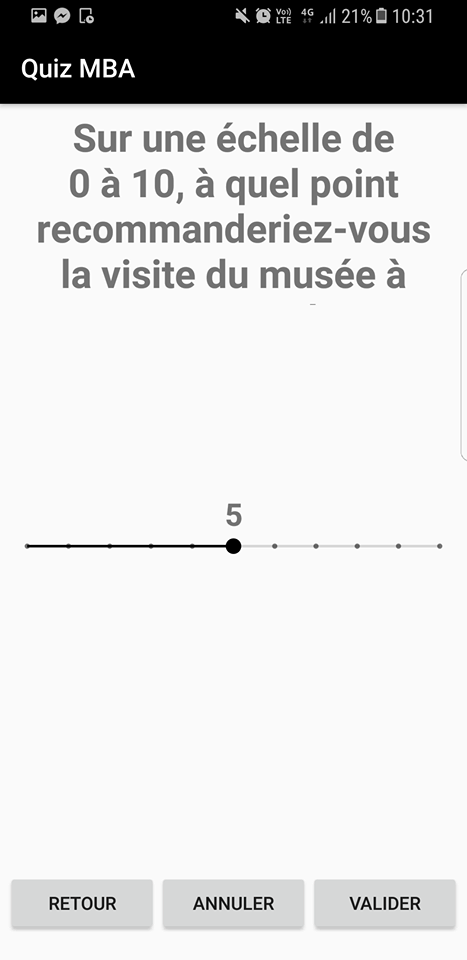
\includegraphics[width=2.8cm]{recommandation.png}
    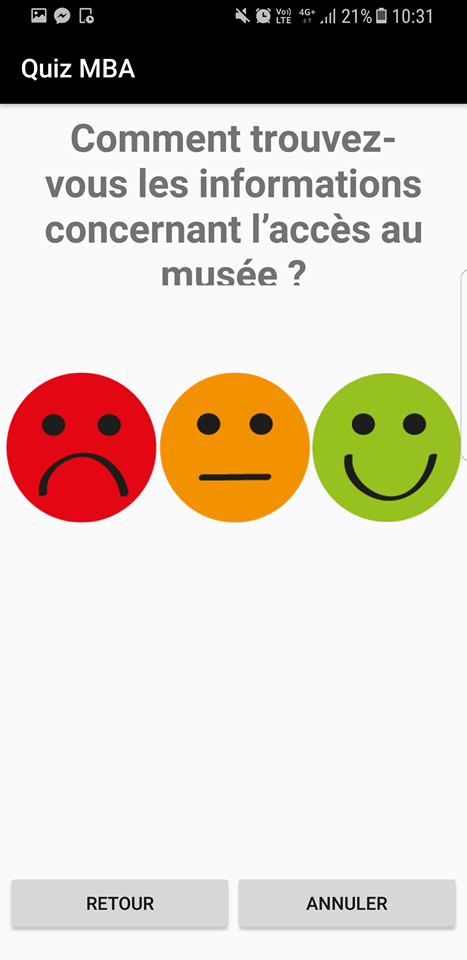
\includegraphics[width=2.8cm]{satisfaction.png}
    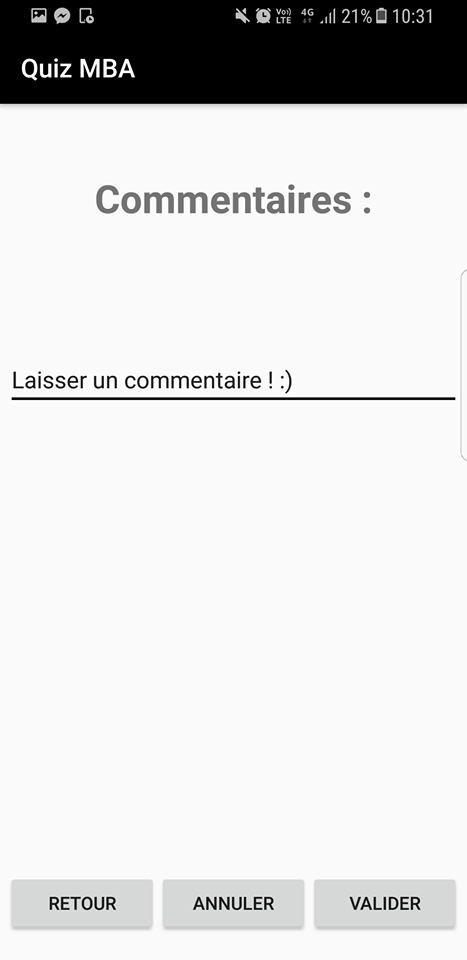
\includegraphics[width=2.8cm]{commentaire.png}
    \captionof{figure}{Illustration des différents types de questions}
  \end{center}

  Les questions ludiques viennent sous la forme de questions sur les oeuvres que le visiteur aura pu voir pendant sa visite.


  \subsection{Implémentation}

  L'application est dirigée par le fichier \emph{Manager.java}. Ce fichier fait le lien entre toutes les questions, ludiques ou non. Ensuite, les données récuppérées par le fichier \emph{request.java} est ensuite envoyé aux fichiers \emph{php}. \par

  Tout le texte utilisé dans les questions est présent dans le fichier \emph{strings.xml}. Toutes les questions et réponses ont un \emph{nom} qui est appelé ensuite dans les différentes activitées. \par

  À chaque question correspond une activitée, ainsi que le menu et la page de fin.
  Dans chaque activité, nous avons une \emph{classe} principale qui contient elle-même quatre \emph{fonctions}: \\
    \begin{itemize}
        \item La fonction \emph{onCreate} qui initialise ce qui va s'inscrire dans la base de données.
        \item La fonction \emph{onStart} qui gère l'interface graphique de la question. C'est cette fonction qui utilise les chaînes de caractères stockées dans \emph{strings.xml}
        \item Les fonctions \emph{nextView} et \emph{previousView} permettant de lier les activités qui contiennent les questions entre elles. \\
    \end{itemize}

  Les fonctions suivantes servent, en plus des autres fonctions, aux question ludiques du questionnaire : \\
  \begin{itemize}
      \item La fonction \emph{verifAnswer} colore le choix du visiteur en vert ou en rouge selon si sa réponse est bonne ou mauvaise.
        \item La fonction \emph{goodAnswer} sert à s'assurer que l'utilisateur a coché toutes les bonnes réponses, lorqu'il y en a plusieurs.

  \end{itemize}
  \section{Administrateur}

  À travers le lien donné dans le manuel d'utilisation (\href{http://sullyvan.tremor.emi.u-bordeaux.fr/script_php/DB_online.php}{ici}), un administrateur peut récupérer
  les informations dont il a besoin en fonction de la période.

  Il sera bien entendu possible de changer la base de données et le site d'exportation pour le Musée des Beaux-Arts.

  \begin{center}
  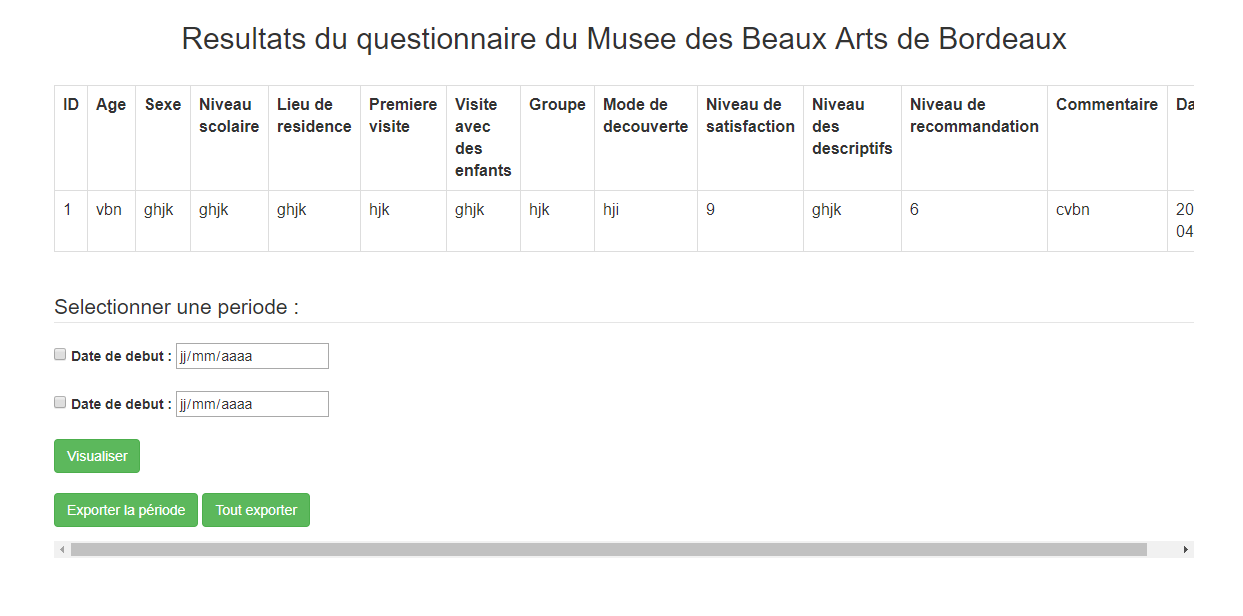
\includegraphics[width=12cm]{bdd.png}
  \captionof{figure}{Exemple de base de données}
  \end{center}

  Il est très facile d'exporter la base de données dans un fichier \emph{Excel}.


  \section{Planning}

  Afin de'orchestrer nos tâches pour le semestre, nous avons organisé nos actions sur le site \emph{Trello}

  \begin{center}
  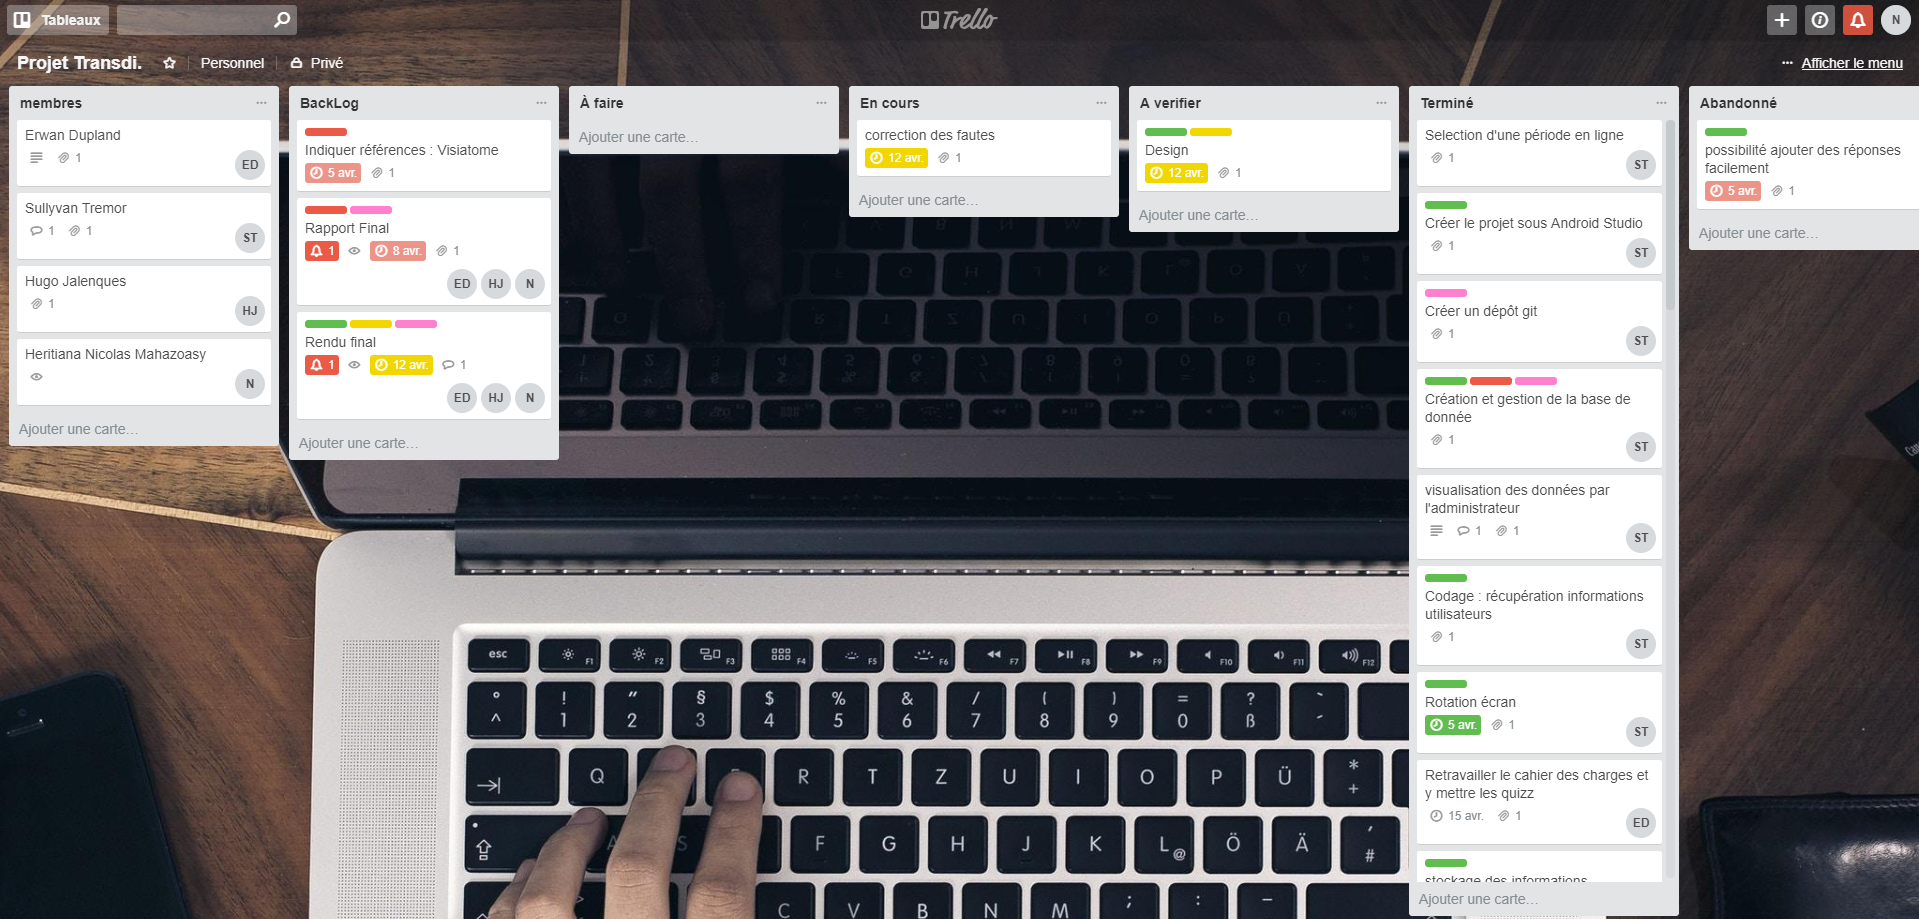
\includegraphics[width=12cm]{trello.png}
  \captionof{figure}{Notre \textbf{Trello} quelques jours avant le rendu final}
  \end{center}

  Nous avons découpé le projet en plusieurs étapes : \emph{Backlog}, \emph{À faire}, \emph{En cours}, \emph{À vérifier} et \emph{Abandonné}. \\

  Nous avons créé un \emph{diagramme de Gantt} pour organiser le travail durant le semestre de manière chronologique grâce aux outils du site \emph{Trello}.
  Grâce au \emph{Trello}, il a été possible de traiter efficacement les différentes tâches à réaliser.
  En cliquant \href{Gantt.pdf}{ici} vous pourrez consulter notre \emph{diagramme de Gantt}.

 \section{Répartition des tâches}

  En lien avec notre tableau \emph{Trello} et notre \emph{diagramme de Gantt}, vous trouverez sur les différentes étiquettes les assignements de tâches de la manière suivante :

  \begin{center}
  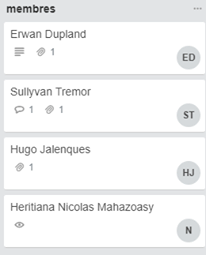
\includegraphics[height=10cm]{membres.png}
  \end{center}
  Voici aussi le lien de notre git : \href{https://services.emi.u-bordeaux.fr/projet/git/pct}{https://services.emi.u-bordeaux.fr/projet/git/pct}
  \newpage
  \section{Contenu de l'archive}

    Dans l'archive que vous avez reçu, vous retrouverez dans son arborescence :
    \begin{itemize}
        \item Un dossier \emph{cdc} contenant notre cahier des charges sur lequel nous avons basé le projet et son déroulement.
        \item Un dossier \emph{comm} contenant les quizz ludiques et leur source pour le quizz ainsi que la question et les réponses correspondantes.
        \item Un dossier \emph{graphic} contenant les codes couleurs du site internet du Musée des Beaux-arts, les logos de ce dernier ainsi que celui du mécène(Haut-Bailly).
        \item Un dossier \emph{QuizzWithServer} contenant tout l'ensemble de l'application: \begin{itemize}
            \item Dans app/src/main/java/com/example/sully/QuizzWithServer vous trouverez l'ensemble de la structure de l'application, notammement la création, la gestion de la base de donnée dans \emph{DatabaseFile}, et de requêtes dans \emph{Requests}.
            \item Dans \emph{PlayfulActivities} vous trouverez toute la partie des questions ludiques du quizz.
            \item Dans \emph{QuestionsActivities} vous trouverez toute la partie des questions essentielles du quizz aux normes internationales de sondage.
        \end{itemize}
        \item Notre diagramme de Gantt.

    \end{itemize}
    \section{Manuel d'utilisation}

  Très simple d'utilisation pour le visiteur, il lui suffit de suivre les instructions et de répondre aux questions du quiz.
  S'il s'arrête en cours de chemin, l'application reviendra à l'accueil en attendant le prochain client.
  Il pourra, depuis l'accueil, préciser la langue dans laquelle il veut remplir le quiz. \\

  L'application n'étant pas hébergée, elle doit être directement transférée d'un pc à une tablette.
  Plusieurs tablettes peuvent utiliser l'application, travaillant sur la même base de données. \\

  Pour l'administrateur, il faudra se rendre sur un site dédié pour récupérer la base de données.
  En cette période de conception, vous trouverez \href{http://sullyvan.tremor.emi.u-bordeaux.fr/script_php/DB_online.php}{ici} l'accès à l'exportateur de la base.

  \chapter{Conclusion}

  Au départ parti sur un tout autre projet durant le premier semestre, \emph{Etude de public} a été pris au second semestre. Nous nous sommes donc retrouvé dans une situation d'indépendance vis-à-vis du projet car nous n'avions que tardivement pu rencontrer notre client, ce qui nous a obligé à nous voir nous-même comme notre propre client, ce qui fut très instructif. \\

  L'objectif du projet était de créer un support informatisé pour le Musée des Beaux-Arts afin qu'ils puisse récupèrer des informations sur leurs visiteurs. Le client voulait un support où le visiteur puisse répondre sincèrement sans être lassé.\\

  Ce projet a été très instructif car il nous a permis de développer une application avec des contraintes apportées par un client.
  De plus, ce projet nous a permis de séparer les tâches de façon productive grâce à \emph{Trello}.
  Ce projet nous a permis de découvrir les "dessous" d'une application, ce que l'utilisateur ne voit pas. \\

  Cependant, nous n'avons pas pu faire une application parfaite car nous avons manqué de temps.
  Nous aurions pû ajouter certaines choses à l'application comme d'autres questions ludiques.
  De plus, notre interface graphique est basique et avec un peu plus de temps, nous aurions peut être pû améliorer notre interface graphique.

\end{document}
